\documentclass[12pt]{article}
\usepackage{amsmath}
\usepackage{amssymb}
\usepackage[letterpaper,top=1.5in,bottom=1.25in,left=0.75in,right=0.75in,centering]{geometry}
\usepackage{fancyhdr}
\usepackage{enumerate}
\usepackage{lastpage}
\usepackage{multicol}
\usepackage{graphicx}
\usepackage{vwcol}
\reversemarginpar

\pagestyle{fancy}
\cfoot{Page \thepage \ of \pageref{LastPage}}\rfoot{{\bf Total Points: 18}}
\chead{MATH 1560}\lhead{Test \#1}

\newcommand{\points}[1]{\marginpar{\hspace{24pt}[#1]}}
\newcommand{\skipline}{\vspace{12pt}}
%\renewcommand{\headrulewidth}{0in}
\headheight 30pt

\newcommand{\di}{\displaystyle}
\newcommand{\abs}[1]{\lvert #1\rvert}
\newcommand{\R}{\mathbb{R}}
\newcommand{\C}{\mathbb{C}}
\renewcommand{\P}{\mathcal{P}}
\DeclareMathOperator{\nul}{null}
\DeclareMathOperator{\range}{range}
\DeclareMathOperator{\spn}{span}
\newcommand{\len}[1]{\lVert #1\rVert}
\newcommand{\Q}{\mathbb{Q}}
\newcommand{\N}{\mathbb{N}}
\renewcommand{\L}{\mathcal{L}}
\newcommand{\dotp}{\boldsymbol{\cdot}}
\newenvironment{amatrix}[1]{%
  \left[\begin{array}{@{}*{#1}{c}|c@{}}
}{%
  \end{array}\right]
}
\newcommand{\bam}{\begin{amatrix}}
\newcommand{\eam}{\end{amatrix}}
\newcommand{\bbm}{\begin{bmatrix}}
\newcommand{\ebm}{\end{bmatrix}}

\begin{document}


\author{Instructor: Sean Fitzpatrick}
\thispagestyle{plain}
\begin{center}
\emph{University of Lethbridge}\\
Department of Mathematics and Computer Science\\
19 September, 2017\\
{\bf MATH 1560 - Test \#1 -- Group Stage}\\
Examiner: Sean Fitzpatrick
\end{center}

\skipline \skipline \skipline \noindent \skipline

Record the names of your group members below. Groups must contain between 3 and 5 members. \\

\textbf{Please print clearly.}

\skipline

\begin{enumerate}
\item Last Name:\underline{\hspace{200pt}} \quad First Name:\underline{\hspace{140pt}}

\skipline\skipline

\item Last Name:\underline{\hspace{200pt}} \quad First Name:\underline{\hspace{140pt}}

\skipline\skipline

\item Last Name:\underline{\hspace{200pt}} \quad First Name:\underline{\hspace{140pt}}

\skipline\skipline

\item Last Name:\underline{\hspace{200pt}} \quad First Name:\underline{\hspace{140pt}}

\skipline\skipline

\item Last Name:\underline{\hspace{200pt}} \quad First Name:\underline{\hspace{140pt}}

\end{enumerate}
%\skipline
%
%\skipline
%Student Number:\underline{\hspace{322pt}}\\
%\skipline



\vspace{0.1in}

\vspace*{\fill}

\begin{quote}
Print your name and student number clearly in the space above. You may remove this cover page, and use the back for scrap paper. If you want any work on the back of this page to be graded, you must clearly indicate this on the page containing the corresponding question.

\medskip

Answer the questions in the space provided. Show all work and necessary justification. Partial credit may be awarded for partially correct work.
 
\medskip

No outside aids are permitted, with the exception of a basic calculator. 
\end{quote}



%\newpage
%\thispagestyle{empty}

%This page left intentionally blank.

\newpage

 \begin{enumerate}
 \item  Evaluate the following limits:
\begin{enumerate}
 \item $\di \lim_{x\to 3} \frac{x^2-6x+9}{x^2-5x+6}$ \points{3}

\vspace{2in}

 \item $\di \lim_{x\to 0}\frac{\tan(7x)}{x}$ \points{3}

\vspace{2in}

 \item $\di \lim_{x\to 1}\frac{\sqrt{x}-1}{x^2-1}$ \points{3} (Suggestion: common denominator.)

\end{enumerate}
\newpage

\item The graph of a function $f$ is given below: \points{9}

\begin{center}
 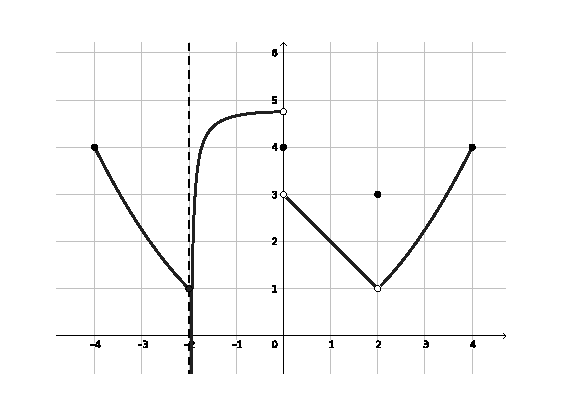
\includegraphics[width=4.5in]{FE-3}
\end{center}


Determine the following values (write DNE if something does not exist):
\begin{multicols}{2}
\begin{enumerate}
 \item The domain of $f$: \underline{\hspace{1in}}
 
 \bigskip
 
 
 \bigskip
 
 \item $\di\lim_{x \to -2^-}f(x)$: \underline{\hspace{1in}}
 
 \bigskip

 \bigskip
 
 \item $\di \lim_{x\to -2^+}f(x)$: \underline{\hspace{1in}}  
 
 \bigskip
 
 \bigskip
 
 \item $\di \lim_{x\to -2}f(x)$: \underline{\hspace{1in}}
 
 \bigskip
 
 \bigskip
 
 \item $f(-2)$: \underline{\hspace{1in}}

\columnbreak


 \item $\di \lim_{x \to 2^-}f(x)$: \underline{\hspace{1in}}
 
 \bigskip
 
 \bigskip
 
 \item $\di \lim_{x\to 2^+}f(x)$: \underline{\hspace{1in}} 

\bigskip

\bigskip

 \item $\di \lim_{x\to 2}f(x)$: \underline{\hspace{1in}}
 
 \bigskip
 
 \bigskip
 
\item $f(2)$: \underline{\hspace{1in}}
\end{enumerate}
\end{multicols}
\end{enumerate}
\end{document}